\documentclass[svgnames,11pt]{beamer}
\input{/home/tof/Documents/Cozy/latex-include/preambule_commun.tex}
\input{/home/tof/Documents/Cozy/latex-include/preambule_beamer.tex}
%\usepackage{pgfpages} \setbeameroption{show notes on second screen=left}
\author[]{Christophe Viroulaud}
\title{Parcours séquentiel}
\date{\framebox{\textbf{Algo 01}}}
%\logo{}
\institute{Première - NSI}
%DODO à faire avant contrôle types construits
\begin{document}
\begin{frame}
    \titlepage
\end{frame}
\begin{frame}
    \frametitle{}
    Le langage Python propose des outils de recherche dans les structures de données:
    \begin{itemize}
        \item \textbf{\texttt{max}}
        \item \textbf{\texttt{min}}
    \end{itemize}
    \begin{framed}
        \centering Peut-on implémenter efficacement les outils natifs de Python?
    \end{framed}

\end{frame}
\section{Algorithme}
\begin{frame}
    \frametitle{Algorithme}

    \begin{center}
        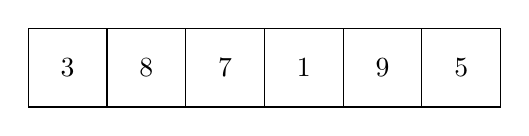
\begin{tikzpicture}
            \draw (0,0) grid (6,1);
            \foreach \x/\n in {0/3,1/8,2/7,3/1,4/9,5/5}{
                    \node at(0.5+\x,0.5) {\n};
                }

        \end{tikzpicture}
        \captionof{figure}{Recherche du maximum}
    \end{center}
    \begin{aretenir}[]
        Pour trouver une valeur dans un tableau il faut le parcourir séquentiellement (élément après élément).
    \end{aretenir}
\end{frame}
\begin{frame}
    \frametitle{}

    \begin{center}
        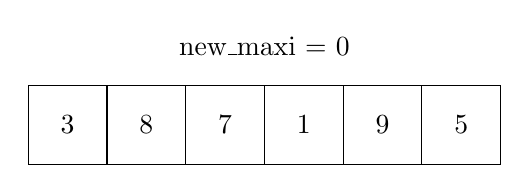
\begin{tikzpicture}
            \draw (0,0) grid (6,1);
            \foreach \x/\n in {0/3,1/8,2/7,3/1,4/9,5/5}{
                    \node at(0.5+\x,0.5) {\n};
                };
            \node at(3,1.5){new\_maxi = 0};
        \end{tikzpicture}
    \end{center}
    \begin{enumerate}
        \item Créer une variable de stockage du maximum provisoire.
    \end{enumerate}
\end{frame}
\begin{frame}
    \frametitle{}

    \begin{center}
        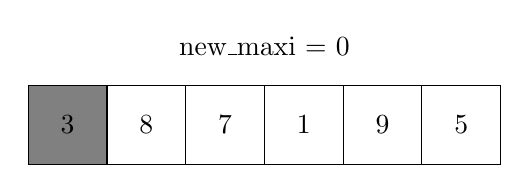
\begin{tikzpicture}
            \fill[gray] (0,0) -- (1,0) -- (1,1) -- (0,1)-- cycle;
            \draw (0,0) grid (6,1);
            \foreach \x/\n in {0/3,1/8,2/7,3/1,4/9,5/5}{
                    \node at(0.5+\x,0.5) {\n};
                };
            \node at(3,1.5){new\_maxi = 0};
        \end{tikzpicture}
    \end{center}
    \begin{enumerate}
        \item Créer une variable de stockage du maximum provisoire.
        \item Comparer la valeur en cours au maximum provisoire et mettre éventuellement à jour ce maximum.
    \end{enumerate}
\end{frame}
\begin{frame}
    \frametitle{}

    \begin{center}
        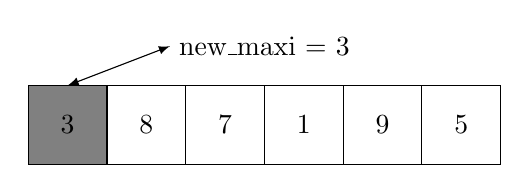
\begin{tikzpicture}
            \fill[gray] (0,0) -- (1,0) -- (1,1) -- (0,1)-- cycle;
            \draw (0,0) grid (6,1);
            \foreach \x/\n in {0/3,1/8,2/7,3/1,4/9,5/5}{
                    \node at(0.5+\x,0.5) {\n};
                };

            \draw[<->,>=latex] (0.5,1) -- (1.8,1.5);
            \node at(3,1.5){new\_maxi = 3};
        \end{tikzpicture}
    \end{center}
    \begin{enumerate}
        \item Créer une variable de stockage du maximum provisoire.
        \item Comparer la valeur en cours au maximum provisoire et mettre éventuellement à jour ce maximum.
    \end{enumerate}
\end{frame}
\begin{frame}
    \frametitle{}

    \begin{center}
        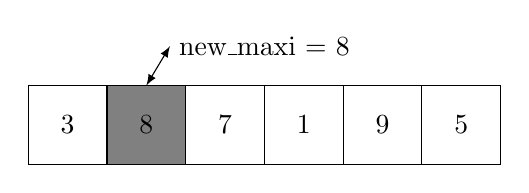
\begin{tikzpicture}
            \fill[gray] (1,0) -- (2,0) -- (2,1) -- (1,1)-- cycle;
            \draw (0,0) grid (6,1);
            \foreach \x/\n in {0/3,1/8,2/7,3/1,4/9,5/5}{
                    \node at(0.5+\x,0.5) {\n};
                };

            \draw[<->,>=latex] (1.5,1) -- (1.8,1.5);
            \node at(3,1.5){new\_maxi = 8};
        \end{tikzpicture}
    \end{center}
    \begin{enumerate}
        \item Créer une variable de stockage du maximum provisoire.
        \item Comparer la valeur en cours au maximum provisoire et mettre éventuellement à jour ce maximum.
        \item Répéter l'étape 2 jusqu'à la fin du tableau.
    \end{enumerate}
\end{frame}
\begin{frame}
    \frametitle{}
    Algorithme de recherche du maximum:
    \begin{enumerate}
        \item Créer une variable de stockage du maximum provisoire.
        \item Comparer la valeur en cours au maximum provisoire et mettre éventuellement à jour ce maximum.
        \item Répéter l'étape 2 jusqu'à la fin du tableau.
    \end{enumerate}
    \begin{activite}
        \begin{enumerate}
            \item Construire par compréhension un tableau de 10 entiers aléatoires compris entre 1 et 100.
            \item Écrire la fonction \textbf{\texttt{maximum(tab: list) $\rightarrow$ int}} qui respecte l'algorithme et renvoie la valeur maximale du tableau.
        \end{enumerate}
    \end{activite}

\end{frame}
\begin{frame}[fragile]
    \frametitle{Correction}

    \begin{center}
        \begin{lstlisting}[language=Python , basicstyle=\ttfamily\small, xleftmargin=2em, xrightmargin=2em]
def maximum(tab: list) -> int:
    """
    valeur maximale de tab

    Args:
        tab (list): tableau

    Returns:
        int: valeur max
    """
    new_maxi = 0
    for val in tab:
        if val > new_maxi:
            new_maxi = val
    # fin de la boucle, renvoie le maxi
    return new_maxi
\end{lstlisting}
        \captionof{code}{Itérer sur le tableau}
        \label{CODE}
    \end{center}

\end{frame}
\begin{frame}[fragile]
    \frametitle{}

    \begin{center}
        \begin{lstlisting}[language=Python , basicstyle=\ttfamily\small, xleftmargin=2em, xrightmargin=2em]
def maximum(tab: list) -> int:
    """
    valeur maximale de tab

    Args:
        tab (list): tableau

    Returns:
        int: valeur max
    """
    new_maxi = 0
    for i in range(len(tab)):
        if tab[i] > new_maxi:
            new_maxi = tab[i]
    # fin de la boucle, renvoie le maxi
    return new_maxi
\end{lstlisting}
        \captionof{code}{Itérer sur les indices}
        \label{CODE}
    \end{center}

\end{frame}
\begin{frame}[fragile]
    \frametitle{}

    \begin{center}
        \begin{lstlisting}[language=Python , basicstyle=\ttfamily\small, xleftmargin=2em, xrightmargin=2em]
# création du tableau
tab = [randint(1, 100) for _ in range(10)]
# affichage du tableau
print(tab)
# affichage du maximum
print(maximum(tab))
\end{lstlisting}
        \captionof{code}{Appel de la fonction}
        \label{CODE}
    \end{center}

\end{frame}
\section{Complexité}
\begin{frame}
    \frametitle{Complexité}

    \begin{aretenir}[]
        Le \textbf{complexité temporelle} représente le nombre d'étapes que l'algorithme doit réaliser pour exécuter sa tâche.
    \end{aretenir}

\end{frame}
\begin{frame}
    \frametitle{}

    \begin{aretenir}[Remarque]
        La durée d'exécution dépend de la puissance de la machine, \underline{mais le nombre d'étapes reste le même}.
    \end{aretenir}

\end{frame}
\begin{frame}
    \frametitle{}

    \begin{center}
        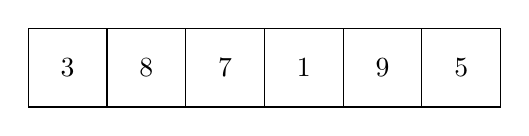
\begin{tikzpicture}
            \draw (0,0) grid (6,1);
            \foreach \x/\n in {0/3,1/8,2/7,3/1,4/9,5/5}{
                    \node at(0.5+\x,0.5) {\n};
                }

        \end{tikzpicture}
        \captionof{figure}{Recherche du maximum}
    \end{center}
    \begin{center}
        Pour trouver le maximum du tableau, l'algorithme doit visiter chaque cellule une fois. Le nombre d'étapes dépend de la taille du tableau.
    \end{center}

\end{frame}
\begin{frame}
    \frametitle{}

    \begin{center}
        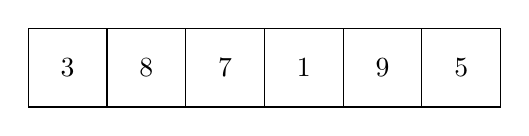
\begin{tikzpicture}
            \draw (0,0) grid (6,1);
            \foreach \x/\n in {0/3,1/8,2/7,3/1,4/9,5/5}{
                    \node at(0.5+\x,0.5) {\n};
                }

        \end{tikzpicture}
        \captionof{figure}{Recherche du maximum}
    \end{center}
    \begin{aretenir}[]
        La complexité de la recherche du maximum d'un tableau dépend de la taille \textbf{\texttt{n}} du tableau. On dit que la complexité est \textbf{linéaire} et on la note:
        $$O(n)$$
    \end{aretenir}

\end{frame}
\begin{frame}
    \frametitle{}

    \begin{activite}
        \begin{enumerate}
            \item Écrire la fonction \textbf{\texttt{est\_present(tab: list, e: int) $\rightarrow$ bool}} qui renvoie \textbf{\texttt{true}} si l'entier \textbf{\texttt{e}} est présent dans le tableau.
            \item Que peut-on dire à propos de la complexité temporelle de cette fonction si l'élément est présent en première position du tableau? En dernière position?
            \item Quelle est la complexité temporelle si l'élément n'est pas présent dans le tableau?
        \end{enumerate}
    \end{activite}

\end{frame}
\begin{frame}[fragile]
    \frametitle{Correction}
    \begin{center}
        \begin{lstlisting}[language=Python , basicstyle=\ttfamily\small, xleftmargin=2em, xrightmargin=2em]
def est_present(tab: list, e: int) -> bool:
    """
    vérifie si e est dans le tableau
    """
    for val in tab:
        if val == e:
            return True
    # On est sorti de la boucle sans avoir trouvé
    return False
\end{lstlisting}
    \end{center}


\end{frame}
\begin{frame}
    \frametitle{}

    \begin{center}
        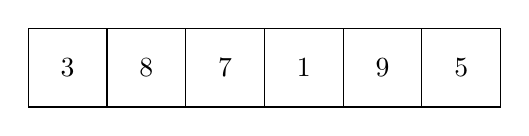
\begin{tikzpicture}
            \draw (0,0) grid (6,1);
            \foreach \x/\n in {0/3,1/8,2/7,3/1,4/9,5/5}{
                    \node at(0.5+\x,0.5) {\n};
                }

        \end{tikzpicture}
    \end{center}
    Complexités:
\begin{itemize}
    \item<1-> \textbf{dans le meilleur des cas:} l'élément cherché est le premier du tableau. La complexité est \textbf{constante} ($O(1)$).
    \item<2-> \textbf{dans le pire des cas:} l'élément cherché n'est pas présent. La complexité est \textbf{linéaire} ($O(n)$).
    \item<3-> \textbf{moyenne:} l'élément est dans le tableau. La complexité est \textbf{linéaire} ($O(n)$).
\end{itemize}
\end{frame}
\section{Terminaison}
\begin{frame}
    \frametitle{Terminaison}
    \begin{aretenir}[]
La \textbf{terminaison} d'un programme est le fait de vérifier qu'il finit par s'arrêter. Dans une boucle on cherche \textbf{un variant de boucle}: une expression qui change à chaque itération, jusqu'à un cas limite.
    \end{aretenir}

    

\end{frame}
\begin{frame}[fragile]
    \frametitle{}

    \begin{center}
        \begin{lstlisting}[language=Python , basicstyle=\ttfamily\small, xleftmargin=2em, xrightmargin=2em]
def maximum(tab: list) -> int:
    new_maxi = 0
    for i in range(len(tab)):
        if tab[i] > new_maxi:
            new_maxi = tab[i]
    # fin de la boucle, renvoie le maxi
    return new_maxi
\end{lstlisting}
        \captionof{code}{La variable \textbf{\texttt{i}} est un variant de la boucle}
        \label{CODE}
    \end{center}   
La variable \textbf{\texttt{i}} augmente à chaque itération. Elle finira toujours par atteindre \textbf{\texttt{len(tab)}}.
\end{frame}
\begin{frame}[fragile]
    \frametitle{}

    \begin{activite}
\begin{center}
\begin{lstlisting}[language=Python , basicstyle=\ttfamily\small, xleftmargin=2em, xrightmargin=2em]
i = 0
while i < 10:
    print(i)
\end{lstlisting}
\end{center}
Ce code termine-t-il?
    \end{activite}

\end{frame}
\begin{frame}
    \frametitle{Correction}

Il n'y a pas de variant de boucle. Le code ne termine pas.

\end{frame}
\begin{frame}[fragile]
    \frametitle{}

    \begin{activite}
\begin{center}
\begin{lstlisting}[language=Python , basicstyle=\ttfamily\small, xleftmargin=2em, xrightmargin=2em]
i = 10
while i != 1:
    if i%2 == 0:
        i = i//2
    else:
        i = 3*i + 1
\end{lstlisting}
\captionof{code}{Suite de Syracuse}
\end{center}
Ce code termine-t-il?
    \end{activite}

\end{frame}
\begin{frame}
    \frametitle{Correction}

Pour \textbf{\texttt{i = 10}} la suite termine. Mais personne n'a encore prouvé que la propriété est vérifiée pour toutes les valeurs de \textbf{\texttt{i}}.   

\end{frame}
\section{Correction}
\begin{frame}
    \frametitle{Correction}

    \begin{aretenir}[]
    La \textbf{correction} d'un programme est le fait de vérifier qu'il réalise effectivement ce qui était prévu. Dans une boucle on cherche \textbf{un invariant de boucle:} une expression qui est vraie avant chaque itération.
    \end{aretenir}

\end{frame}
\begin{frame}[fragile]
    \frametitle{}

    \begin{center}
        \begin{lstlisting}[language=Python , basicstyle=\ttfamily\small, xleftmargin=2em, xrightmargin=2em]
def maximum(tab: list) -> int:
    new_maxi = 0
    for i in range(len(tab)):
        if tab[i] > new_maxi:
            new_maxi = tab[i]
    # fin de la boucle, renvoie le maxi
    return new_maxi
\end{lstlisting}
        \captionof{code}{\centering \guill{\textbf{\texttt{new\_maxi contient le maximum du début du tableau}}} est un invariant.}
        \label{CODE}
    \end{center}   

\end{frame}
\begin{frame}
    \frametitle{}

    \begin{center}
        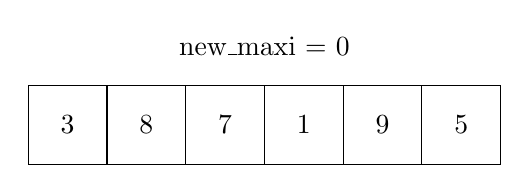
\begin{tikzpicture}
            
            \draw (0,0) grid (6,1);
            \foreach \x/\n in {0/3,1/8,2/7,3/1,4/9,5/5}{
                    \node at(0.5+\x,0.5) {\n};
                };

            \node at(3,1.5){new\_maxi = 0};
        \end{tikzpicture}
    \end{center}
\begin{itemize}
    \item Avant la première itération, la propriété est vraie.
\end{itemize}
\end{frame}
\begin{frame}
    \frametitle{}

    \begin{center}
        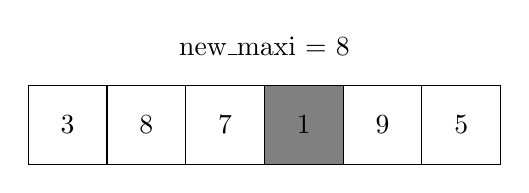
\begin{tikzpicture}
            \fill[gray] (3,0) -- (4,0) -- (4,1) -- (3,1)-- cycle;
            \draw (0,0) grid (6,1);
            \foreach \x/\n in {0/3,1/8,2/7,3/1,4/9,5/5}{
                    \node at(0.5+\x,0.5) {\n};
                };

            \node at(3,1.5){new\_maxi = 8};
        \end{tikzpicture}
    \end{center}
\begin{itemize}
    \item Avant la première itération, la propriété est vraie.
    \item On suppose que la propriété est vraie pour l'itération \textbf{\texttt{n}}.
\end{itemize}
\end{frame}
\begin{frame}
    \frametitle{}

    \begin{center}
        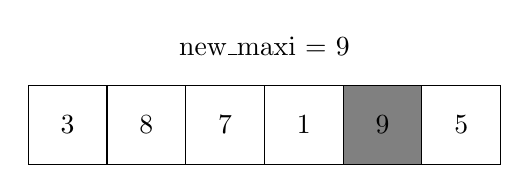
\begin{tikzpicture}
            \fill[gray] (4,0) -- (5,0) -- (5,1) -- (4,1)-- cycle;
            \draw (0,0) grid (6,1);
            \foreach \x/\n in {0/3,1/8,2/7,3/1,4/9,5/5}{
                    \node at(0.5+\x,0.5) {\n};
                };

            \node at(3,1.5){new\_maxi = 9};
        \end{tikzpicture}
    \end{center}
\begin{itemize}
    \item Avant la première itération, la propriété est vraie.
    \item On suppose que la propriété est vraie pour l'itération \textbf{\texttt{n}}.
    \item À l'itération suivante \textbf{\texttt{new\_maxi}} est comparé et mis à jour.
\end{itemize}
\end{frame}
\end{document}